\begin{center}

  \begin{tabular}{rp{6cm}lp{12cm}}%{rl}

  % after \\: \hline or \cline{col1-col2} \cline{col3-col4} ...

  论文地址:& \href{https://openreview.net/pdf?id=R3a2G2tSf3c}{https://openreview.net/pdf?id=R3a2G2tSf3c} \\

  %源码:& \href{xxx}{xxx} \\

%  slides:& \href{http://yunshengb.com/wp-content/uploads/2017/03/nips_2018_r2l_workshop_talk.pdf}{{\footnotesize Convolutional Set Matching for Graph Similarity}}\\

  关键词:& \textbf{Graph Similarity, Graph Classification, Metric Learning} \\

  写于:& \date{2020-10-15}

  \end{tabular}

\end{center}

该论文针对图分类问题提出了新的解决方案 --- Graph-Graph(G2G)。现有的图分类方法中,通常会忽略图数据之间的关系 --- 当然图数据之间也没有直观的联系。论文中以图为结点,图之间的相似性为边的权重构建了 SuperGraph,之后图的分类问题则转变成SuperGraph中结点分类的问题。G2G方法过程如Fig.\ref{fig:G2G}所示。

\begin{figure}[h]
	\centering
	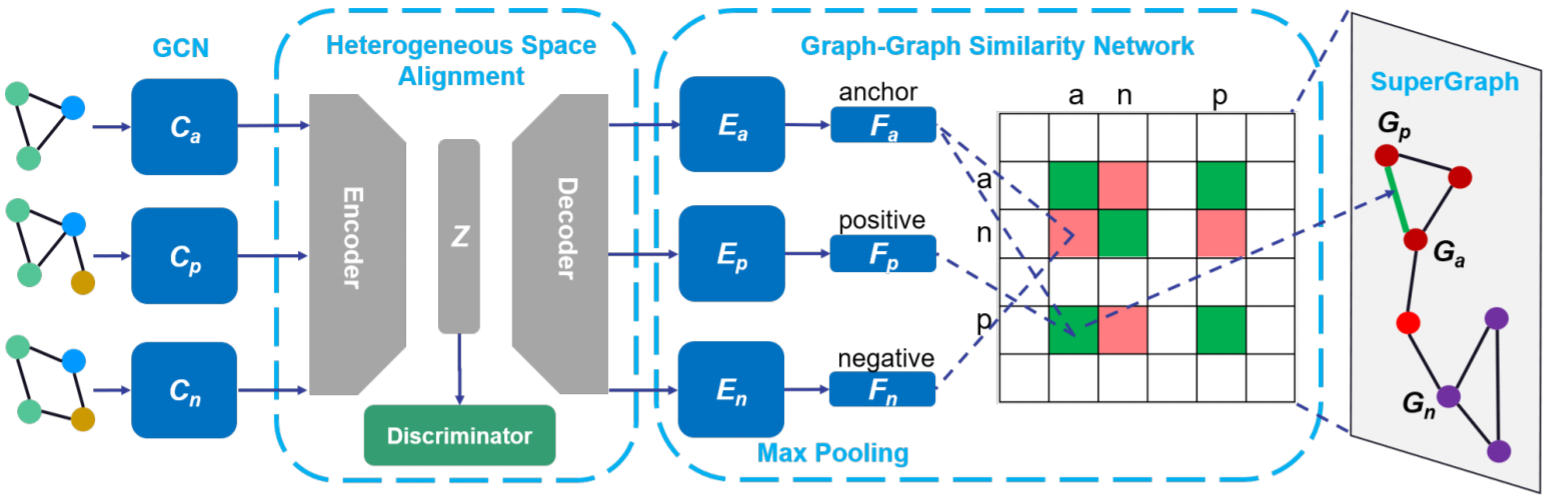
\includegraphics[width=.8\textwidth]{pics/G2G}
	\caption{Overview of Graph-Graph}
	\label{fig:G2G}
\end{figure}

\paragraph{G2G思路}如Fig.\ref{fig:G2G}所示,G2G可以分为四个部分:
\subparagraph{GCN}使用一个共享的GCN为所有的图的结点生成表征。

\subparagraph{Heterogeneous Space Alignment}使用对抗自动编码器\cite{makhzani2016adversarial}用于对生成表征对齐到同一个空间。\tred{这也是我的一个问题,不同的图中的结点的表征所在的空间之间有什么联系呢?}

\subparagraph{Graph-Graph Similarity Network}先通过一个Max pooling来得到图的表征,再基于Contrastive loss和Triplet loss,使用NN来学习图之间的相似性。

\subparagraph{SuperGraph}基于图的表征和相似性矩阵构建一个SuperGraph,每个图都是一个结点,相似性为边的权重。再图表征的基础上,可以使用传统的机器学习方法对SuperGraph中的结点 --- 即原来的图进行分类,论文中使用的是KNN对结点进行分类。
\newline

有一点要注意,G2G每次都使用3个图作为输入,分别是anchor,positive,negative,anchor和positive之间是同类的图,anchor和negative之间是不同类的图,因此在训练过程中使用了Contrastive loss和Triplet loss。

\paragraph{方法解决的问题/优势}
\begin{itemize}
	\item 在完成图分类任务的过程中,学习到了图之间的相似性
	\item 挖掘图的表征空间之间的关系,针对表征空间的问题提出了解决方案,将不同图的表征进行了对齐(\tbc{red}{还有点不太理解文中的意思,原文是:align all the graphs to a same distribution)}
	\item 在对graph-level进行分类时,考虑了图之间的关系(similarity)
	\item 使用triplet进行寻来
\end{itemize}

\paragraph{方法的局限性/未来方向}
\begin{itemize}
	\item 在图类别较多的数据集上效果不是很好
	\item 现有的图分类方法中,主要考虑的是结点的特征和图的拓扑结构,实际中\tbc{red}{边在图中也有很大的作用},进行进行graph-level的任务时,能否考虑边的信息

\end{itemize}


虽然这篇论文还在双盲中,但我怀疑这篇论文又是\href{http://yunshengb.com/}{Yunsheng Bai}做的。



